\section{Model and the External Population}

The model described until this point observed only the process inside the closed population of a hospital. In reality, it is almost impossible to imagine a self-sustaining hospital that does not have any connection to the external world. People are going inside and outside of any real-life hospital, therefore the mathematical model should also account for that. The individuals going in and out of the hospital may not only be patients, but also the medical personnel.

The first element to be created is the stock representing the external world. Since the external society is not in our interest, we can just simplify it to a single stock. We call it Society. Any flow going outside of the hospital will head to the Society stock and any flow coming to the system from outside will come from this stock, too. The value of the Society will change during simulation, so we will initialize it using a TotalPopulation parameter.

\begin{figure}[H]
  \centering
  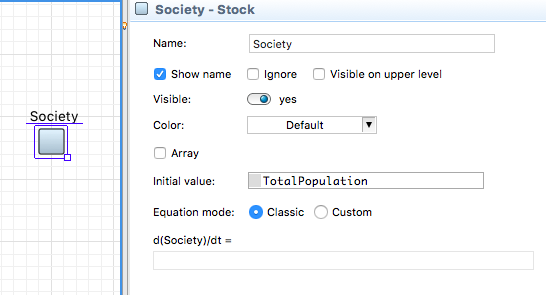
\includegraphics[height=0.4\textwidth]{img/screens/society/society1}
  \caption{The Society stock and its properties}
\end{figure}

The parameters that we were using in previous chapters will help to define the initial value for Society, too. TotalPopulation is a parameter, which will have a symbolic value of 100000. This is an approximation of a small town population.

\begin{figure}[H]
  \centering
  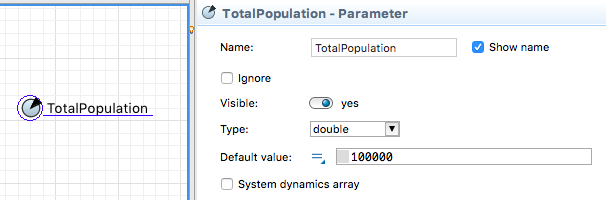
\includegraphics[height=0.3\textwidth]{img/screens/society/society2}
  \caption{The setting of TotalPopulation parameter}
\end{figure}

In order to use the TotalPopulation parameter in the Society stock value, we need to draw some connection between them. This is the way we used to bind parameters to other objects, like stocks.

\begin{figure}[H]
  \centering
  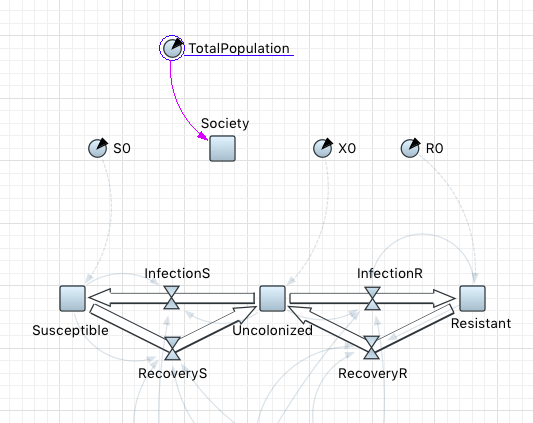
\includegraphics[height=0.5\textwidth]{img/screens/society/society3}
  \caption{Linking the Society and TotalPopulation in the model}
\end{figure}

The next step is to create the first flow from Society stock. EnterS flow will go from Society to Susceptible, indicating the incoming individuals colonized by susceptible strain of the bacteria.

\begin{figure}[H]
  \centering
  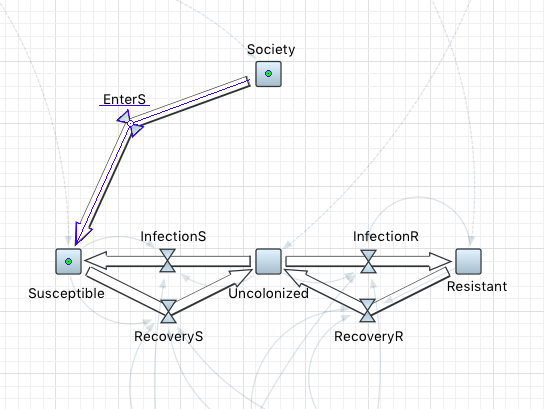
\includegraphics[height=0.5\textwidth]{img/screens/society/society7}
  \caption{The flow of EnterS}
\end{figure}

The value of the EnterS flow will depend on two more parameters that we are going to create next. As it is seen from the corresponding figure, we are setting the value of EnterS to $\mu m$.

\begin{figure}[H]
  \centering
  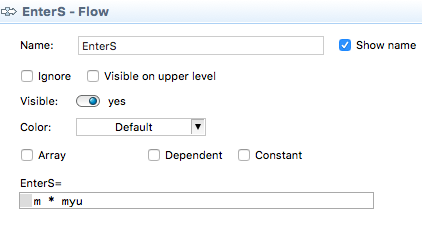
\includegraphics[height=0.3\textwidth]{img/screens/society/society16}
  \caption{The properties of EnterS flow}
\end{figure}

In order to indicate the number of individuals entering the hospital from Society into different categories, we need to create a parameter $m$. This variable is a fraction of incoming people that are colonized with susceptible bacteria. The value of it may differ from one disease to another, but we set a symbolic value of 0.3 to it.

\begin{figure}[H]
  \centering
  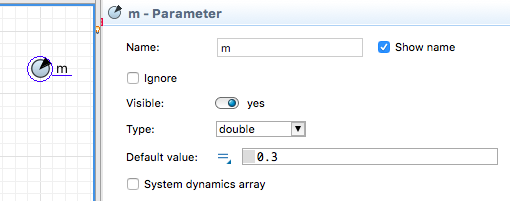
\includegraphics[height=0.3\textwidth]{img/screens/society/society4}
  \caption{The properties of parameter $m$}
\end{figure}

Another parameter that is necessary for the flows of people is $\mu$. This variable indicates the total number of individuals entering the hospital daily. This number also provides the average length of stay in the hospital, which is equal to $1/\mu$. We set the value of this parameter to 0.1.

\begin{figure}[H]
  \centering
  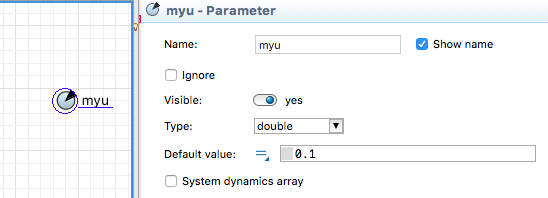
\includegraphics[height=0.3\textwidth]{img/screens/society/society6}
  \caption{The parameter $\mu$ and its properties}
\end{figure}

After creating the mentioned parameters, we can add them to our model. The amount of different interactive elements of the model is increasing, so it is a good practice to keep things separated. We put the parameters near the other ones.

\begin{figure}[H]
  \centering
  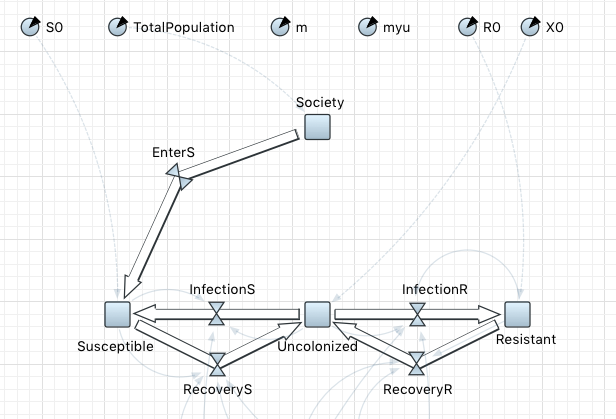
\includegraphics[height=0.5\textwidth]{img/screens/society/society5}
  \caption{Placing $m$ and $\mu$ in the model}
\end{figure}

Since both parameters that we created are used in the value expression of the flow of incoming individuals infected with susceptible bacteria, we will need to connect the parameters with the flow element.

\begin{figure}[H]
  \centering
  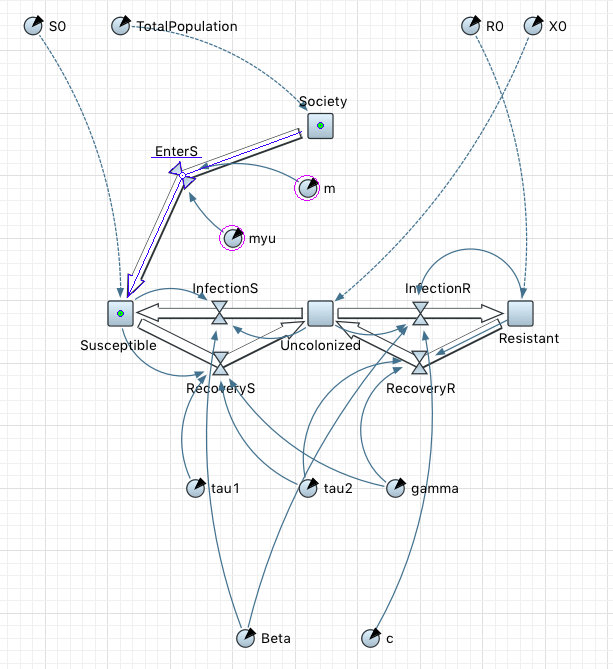
\includegraphics[height=0.6\textwidth]{img/screens/society/society8}
  \caption{Binding $m$ and $\mu$ to the EnterS flow}
\end{figure}

It is necessary to mention that not all of the entering individuals are colonized with bacteria. Therefore, we create a flow of people from Society stock to the Uncolonized stock.

\begin{figure}[H]
  \centering
  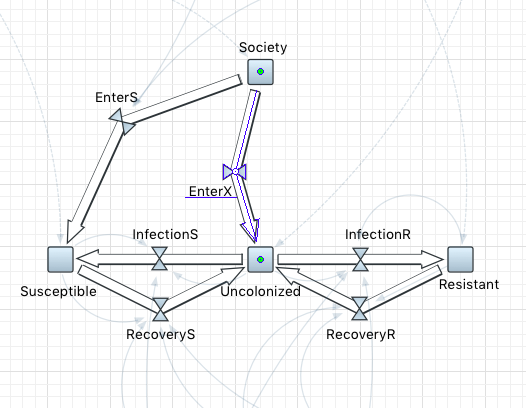
\includegraphics[height=0.5\textwidth]{img/screens/society/society9}
  \caption{The flow of entering individuals uncolonized with bacteria}
\end{figure}

The value of the EnterX flow is different from that of EnterS by only one coefficient - it is $(1 - m)$ instead of $m$. The values of these two flows sum up to $\mu$.

\begin{figure}[H]
  \centering
  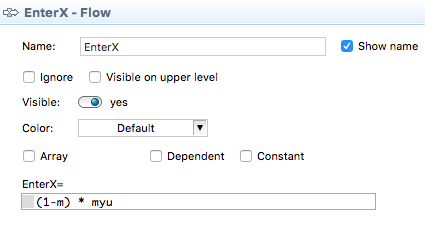
\includegraphics[height=0.3\textwidth]{img/screens/society/society17}
  \caption{Properties of the EnterX flow}
\end{figure}

Like in the case of EnterS, the expession indicating the value of EnterX also uses parameters $m$ and $\mu$. This is why we need to connect the parameters with the EnterX flow to enable the referencing of variables. Each of the parameters has two bindings after this.

\begin{figure}[H]
    \centering
    \begin{subfigure}[b]{0.48\textwidth}
        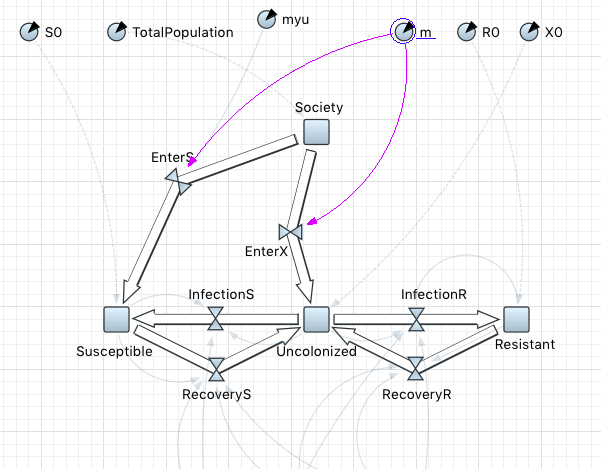
\includegraphics[width=\textwidth]{img/screens/society/society10}
        \caption{The connections of parameter $m$}
    \end{subfigure}
    ~ %add desired spacing between images, e. g. ~, \quad, \qquad, \hfill etc.
      %(or a blank line to force the subfigure onto a new line)
    \begin{subfigure}[b]{0.48\textwidth}
        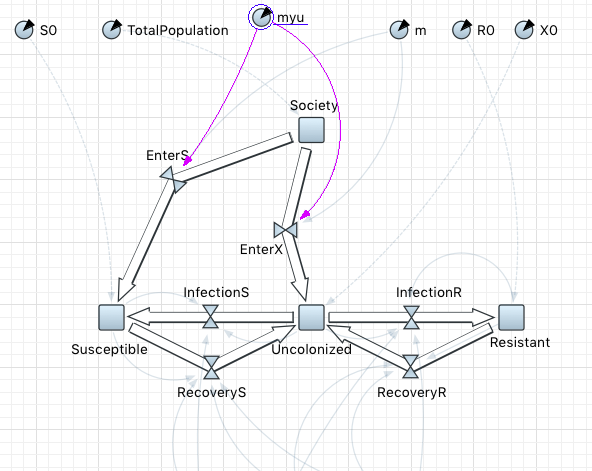
\includegraphics[width=\textwidth]{img/screens/society/society11}
        \caption{The connections of parameter $\mu$}
    \end{subfigure}
    \caption{Binding parameters to EnterX flow}
\end{figure}

A logically symmetric event for the incoming flow of people is departure from hospital. Each of the observed groups of people is going to have its own outgoing flow. As an example the following figure demonstrates the creation of LeaveS flow.

\begin{figure}[H]
  \centering
  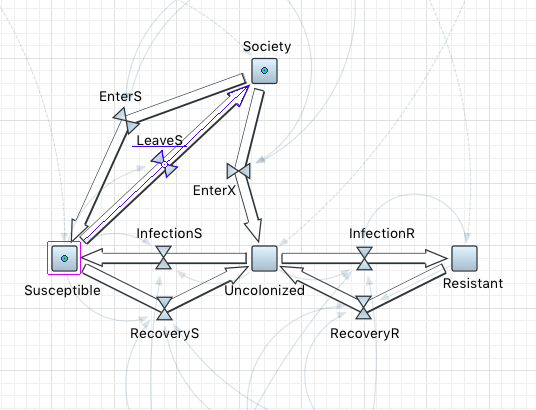
\includegraphics[height=0.5\textwidth]{img/screens/society/society12}
  \caption{Creation of LeaveS flow}
\end{figure}

The value of LeaveS flow depends on the number of population infected by susceptible strain and the parameter $\mu$. The value is going to be $\mu \cdot Susceptible$.

\begin{figure}[H]
  \centering
  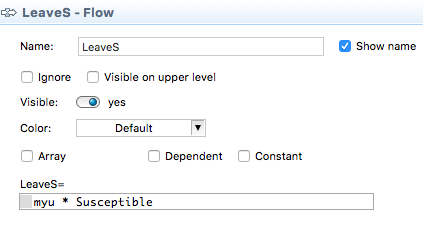
\includegraphics[height=0.3\textwidth]{img/screens/society/society18}
  \caption{The properties of LeaveS flow}
\end{figure}

To provide a correct referencing of the $\mu$ parameter, we need to create a connection between it and the current flow. As it can be seen from the figure, the parameter has now a new connection.

\begin{figure}[H]
  \centering
  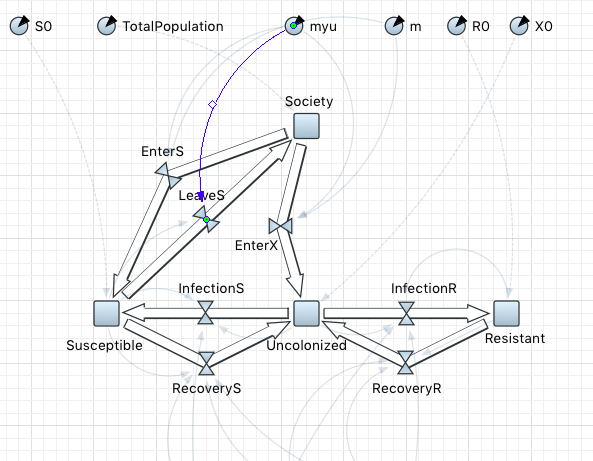
\includegraphics[height=0.5\textwidth]{img/screens/society/society13}
  \caption{Including $\mu$ parameter for the LeaveS flow}
\end{figure}

Similar to LeaveS, we create the corresponding flows for the population colonized with resistant bacteria and uncolonized group. The expression for them will be equal to $\mu \cdot Resistant$ and $\mu \cdot Uncolonized$ respectively.

\begin{figure}[H]
  \centering
  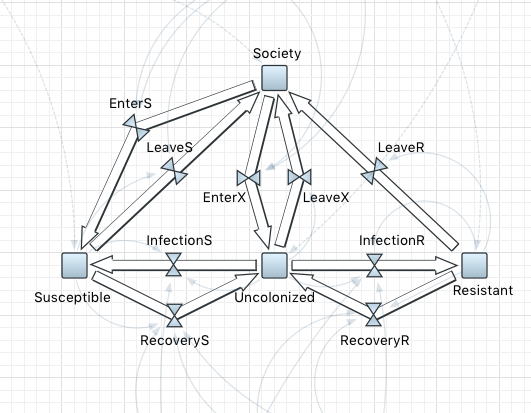
\includegraphics[height=0.5\textwidth]{img/screens/society/society15}
  \caption{Addition of flows of uncolonized and resistant strain departures}
\end{figure}

As it was with LeaveS, the other two new flows also need to reference the $\mu$ parameter and corresponding stock values. Hence we create the neccessary connection between the objects in the model.

\begin{figure}[H]
  \centering
  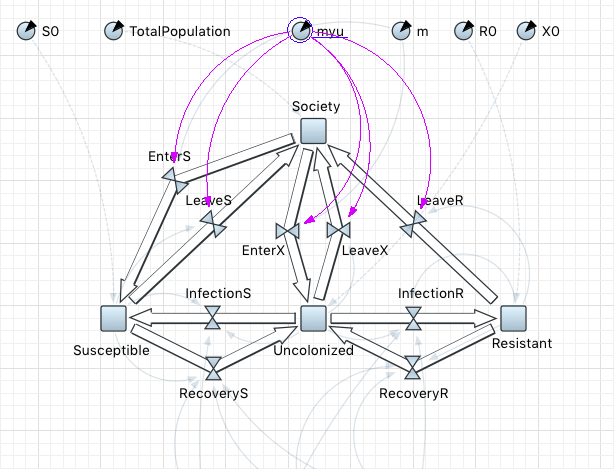
\includegraphics[height=0.5\textwidth]{img/screens/society/society14}
  \caption{Parametrization of LeaveS, LeaveR and LeaveX flows}
\end{figure}

When we finally have added all of the entering and leaving flows and connected them with the necessary parameters, we obtain the model with a Society stock. Now our model has its way of interaction with the external world, individuals come from the outside and leave there. The model is almost ready at this point.

\begin{figure}[H]
  \centering
  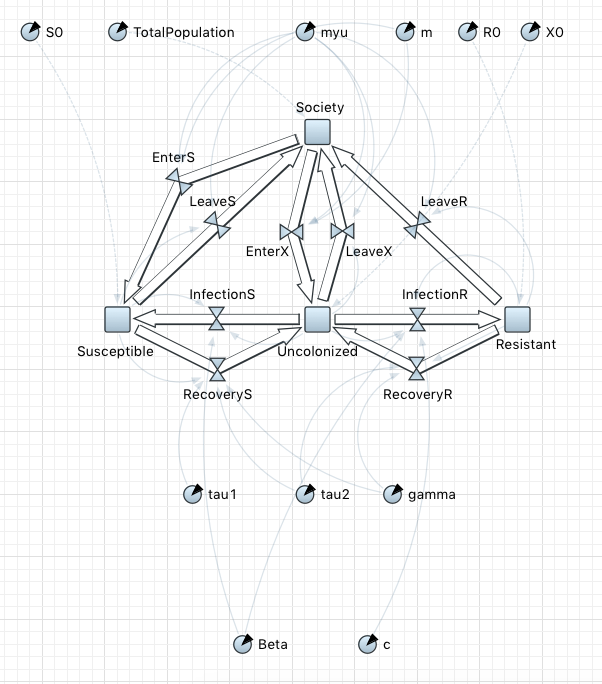
\includegraphics[height=0.6\textwidth]{img/screens/society/society21}
  \caption{The model with completed external interactions}
\end{figure}

In the next sections we are going to add some additional controls to the model in order to enable convenient environment for simulation. The analysis and interpretation of the simulation results would also benefit from the added features.